
%(BEGIN_QUESTION)
% Copyright 2007, Tony R. Kuphaldt, released under the Creative Commons Attribution License (v 1.0)
% This means you may do almost anything with this work of mine, so long as you give me proper credit

Discharge pressure for a compressor may be controlled by throttling the suction line, like this:

$$\includegraphics[width=15.5cm]{i01786x01.eps}$$

Limits must be placed on this pressure control system, however, to avoid damaging the compressor and/or the driving motor under certain operating conditions.  In conditions where there is low discharge flow (i.e. reduced demand for compressed gas) and the pressure controller tries to keep discharge pressure from rising too high by closing off the suction valve, suction pressure may drop below atmospheric, causing ``gland sealing'' oil to be sucked into the compressor.  This can cause damage to the compressor, so a vacuum condition on the suction line should be avoided.  However, the pressure controller knows nothing of the suction line pressure, and so cannot police itself from entering this range of operation.

Conversely, when gas demand is high and the pressure controller opens up the suction valve wide to maintain adequate discharge pressure, the electric motor may become overloaded.  Once again, this can cause damage, and once again the pressure controller is ignorant of motor load and so cannot prevent it from happening.

\vskip 10pt

With the addition of two more controllers and a couple of select relays, though, both problems may be avoided.  This is called {\it override control}:

$$\includegraphics[width=15.5cm]{i01786x02.eps}$$

Identify the proper action (direct or reverse) of each controller, and explain how this override control system functions.

\vskip 20pt \vbox{\hrule \hbox{\strut \vrule{} {\bf Suggestions for Socratic discussion} \vrule} \hrule}

\begin{itemize}
\item{} Explain what will happen in this system if the suction pressure transmitter fails with a low signal (indicating maximum suction).
\item{} Explain what will happen in this system if the power transmitter fails with a low signal (indicating an idling motor).
\item{} Explain what will happen in this system if the discharge pressure transmitter fails with a low signal (indicating low output pressure).
\end{itemize}

\underbar{file i01786}
%(END_QUESTION)





%(BEGIN_ANSWER)

The power controller (JIC) ensures the suction valve can never open up far enough to overload the motor, while the suction pressure controller ensures the suction valve can never close off far enough to draw sealing oil into the compressor.

$$\includegraphics[width=15.5cm]{i01786x03.eps}$$

%(END_ANSWER)





%(BEGIN_NOTES)

The high-select relay ensures a minimum suction valve opening based on suction line pressure, while the low-select relay ensures a maximum suction valve opening based on motor load.

\vskip 30pt

Note: this control strategy derived from diagram on page 130 of Francis G. Shinskey's {\it Energy Conservation Through Control}, copyright 1978.

\vfil \eject

\noindent
{\bf Summary Quiz:}

Identify a fault that could cause the compressor's suction valve to fully open (100\%), assuming all transmitters are direct-acting and the valve is signal-to-open:

$$\includegraphics[width=15.5cm]{i01786x02.eps}$$

\begin{itemize}
\item{} JT fails with a high (20 mA) signal
\vskip 5pt 
\item{} Discharge PT fails with a high (20 mA) signal
\vskip 5pt 
\item{} Signal line to valve fails open (0 mA)
\vskip 5pt 
\item{} Suction PT fails with a low (4 mA) signal
\vskip 5pt 
\item{} Suction PT fails with a high (20 mA) signal
\end{itemize}


%INDEX% Control, strategies: override control
%INDEX% Process: compressor load control
%INDEX% Relay, computational: symbol identification

%(END_NOTES)


